\chapter{Two step RSB}

In this chapter I will investigate the two step RSB structure that is formally similar to the recursion relation found in the one RSB scheme. This will be executed by doing exactly the same steps as in one RSB solution, but this time using the one RSB solution itself as a starting point.

\section{From one to two steps}

I will divide each possible state $\alpha$ of the system into a large number of substates, each now labeled by $\gamma$ similarly to what we've done at a 1 step level. Let now $N_c$ be the number of states, and $N_s$ the number of substates, i.e. the number of states within a state.

It is possible to visualize this hierarchy pictorially using a tree-like structure.

\begin{figure}[t]
\centering
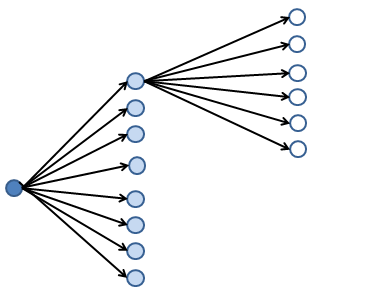
\includegraphics{img/twostep.png}
\caption{Two step RSB, states and substates are organized hierarchically}
\label{fig:2rsb}
\end{figure}

We assume now that each field distribution is independent from the one in other states or clusters.
In order to avoid confusion, the state level will be called \'Cluster level\', and the substate level will now be called
the \'state level\'.

\begin{equation}
Q_0(\emph{h})=\prod_\alpha Q(\emph{h}^\alpha)
\end{equation}

\begin{equation}
Q_0({\emph{h}^\alpha})=\prod_\gamma Q(h^{\alpha\gamma})
\end{equation}

Each state $\gamma$ has a proper weight that follows an exponential distribution. Similarly to what happens in one step RSB we can write
\begin{equation}
\rho(F^{\alpha\gamma}) = \exp(\beta x_s (F^{\alpha\gamma}-{F}^{\alpha}))
\label{distro2}
\end{equation}

Each cluster $\alpha$ has a proper weight that follows an exponential distribution too.
\begin{equation}
\rho(F^\alpha) = \exp(\beta x_C (F^\alpha-{F_R}))
\label{distro1}
\end{equation}

We will call $x_C$ the $x$ variable at a cluster level, in order to distinguish it from $x_s$, the $x$ variable at a state level. 